\documentclass[conference]{IEEEtran}
\IEEEoverridecommandlockouts
% The preceding line is only needed to identify funding in the first footnote. If that is unneeded, please comment it out.
\usepackage{cite}
\usepackage{amsmath,amssymb,amsfonts}
\usepackage{algorithmic}
\usepackage{graphicx}
\usepackage{textcomp}
\usepackage{xcolor}
\usepackage{multirow}
\def\BibTeX{{\rm B\kern-.05em{\sc i\kern-.025em b}\kern-.08em
    T\kern-.1667em\lower.7ex\hbox{E}\kern-.125emX}}
\begin{document}

\title{Use Rate Prediction For Charging Stations\\}

\author{\IEEEauthorblockN{1\textsuperscript{st} Given Name Surname}
\IEEEauthorblockA{\textit{dept. name of organization (of Aff.)} \\
\textit{name of organization (of Aff.)}\\
City, Country \\
email address}
\and
\IEEEauthorblockN{2\textsuperscript{nd} Given Name Surname}
\IEEEauthorblockA{\textit{dept. name of organization (of Aff.)} \\
\textit{name of organization (of Aff.)}\\
City, Country \\
email address}
\and
\IEEEauthorblockN{3\textsuperscript{rd} Given Name Surname}
\IEEEauthorblockA{\textit{dept. name of organization (of Aff.)} \\
\textit{name of organization (of Aff.)}\\
City, Country \\
email address}
\and
\IEEEauthorblockN{4\textsuperscript{th} Given Name Surname}
\IEEEauthorblockA{\textit{dept. name of organization (of Aff.)} \\
\textit{name of organization (of Aff.)}\\
City, Country \\
email address}
\and
\IEEEauthorblockN{5\textsuperscript{th} Given Name Surname}
\IEEEauthorblockA{\textit{dept. name of organization (of Aff.)} \\
\textit{name of organization (of Aff.)}\\
City, Country \\
email address}
\and
\IEEEauthorblockN{6\textsuperscript{th} Given Name Surname}
\IEEEauthorblockA{\textit{dept. name of organization (of Aff.)} \\
\textit{name of organization (of Aff.)}\\
City, Country \\
email address}
}

\maketitle

\begin{abstract}
This paper provides a time frame based prediction model for use rate of charging stations in Shanghai. The approach proposed in this paper takes both station's geographical information and working elements including price and type, into consideration, aimed to classify whether it's a high-use-rate station or a low-use-rate one during different time periods. Experimental results show that our method performs well on LR, Random Forest, SVM and XGBOOST.
\end{abstract}

\begin{IEEEkeywords}
time frame, use rate, charging station, geographical information, POIs
\end{IEEEkeywords}

\section{Introduction}
An electric vehicle charging station, also called EV charging station is an element in an infrastructure that supplies electric energy for the recharging of electric vehicles, such as plug-in electric vehicles and plug-in hybrids. At home or work, some electric vehicles have onboard converters that can plug into a standard electrical outlet or a high-capacity appliance outlet. 

However, in most cases, others require a charging station that provides electrical conversion, monitoring, or safety functionality. These stations are also needed when travelling, and many support faster charging at higher voltages and currents than are available from residential EVSEs. Public charging stations are typically on-street facilities provided by electric utility companies or located at retail shopping centers and operated by many private companies.

EVs in China is experiencing an overall growth in the past few years, which directly results in the massive construction and modification of charging stations and current road networks. However, the cost of construction of charging stations is considerable and are often very costly or even impracticable to reallocate. This raise the question of how to select the locations for building the charging stations.

In a typical view, a charging station no matter where it is located, its 'success' is often determined by the use rate of a station.  

In order to help with station setting strategies, we explore a time frame based prediction model to classify stations into high use-rate and low-use-rate in various time frames, using features like georaphical information as well as other working elements.

We evaluate our method on RL, Random Forest, SVM and XGBOOST, which achieve relatively satisfactory results.

\section{Problem Definition}

It's a binary classification problem. The aim is to predict that one station is of high use rate or low use rate according to its georaphical information and working elements during different time periods.

\section{Related Work}
Hence, we studied the optimization problem of how to deploy charging stations. Existing works \cite{b1} mainly falls into the domain of bike-sharing. Current works of location selection are usually based on the flow prediction of a single station. Futhermore, they rely heavily on the historical data. We argue that the surrounding point of interests as well as distances to important POIs(e.g, metro stations, estates, etc.) play an important role in selecting the optimal location for stations.

\section{Feature Description}

\subsection{Feature Extraction}
From the data we gathered, we made several observations that benefits the features to be included in the model we present. We separate the data into different time frames in order to determine the overall difference among them, since charging network is a dynamic system.
\begin{figure}
	\begin{tabular}{ccc}
		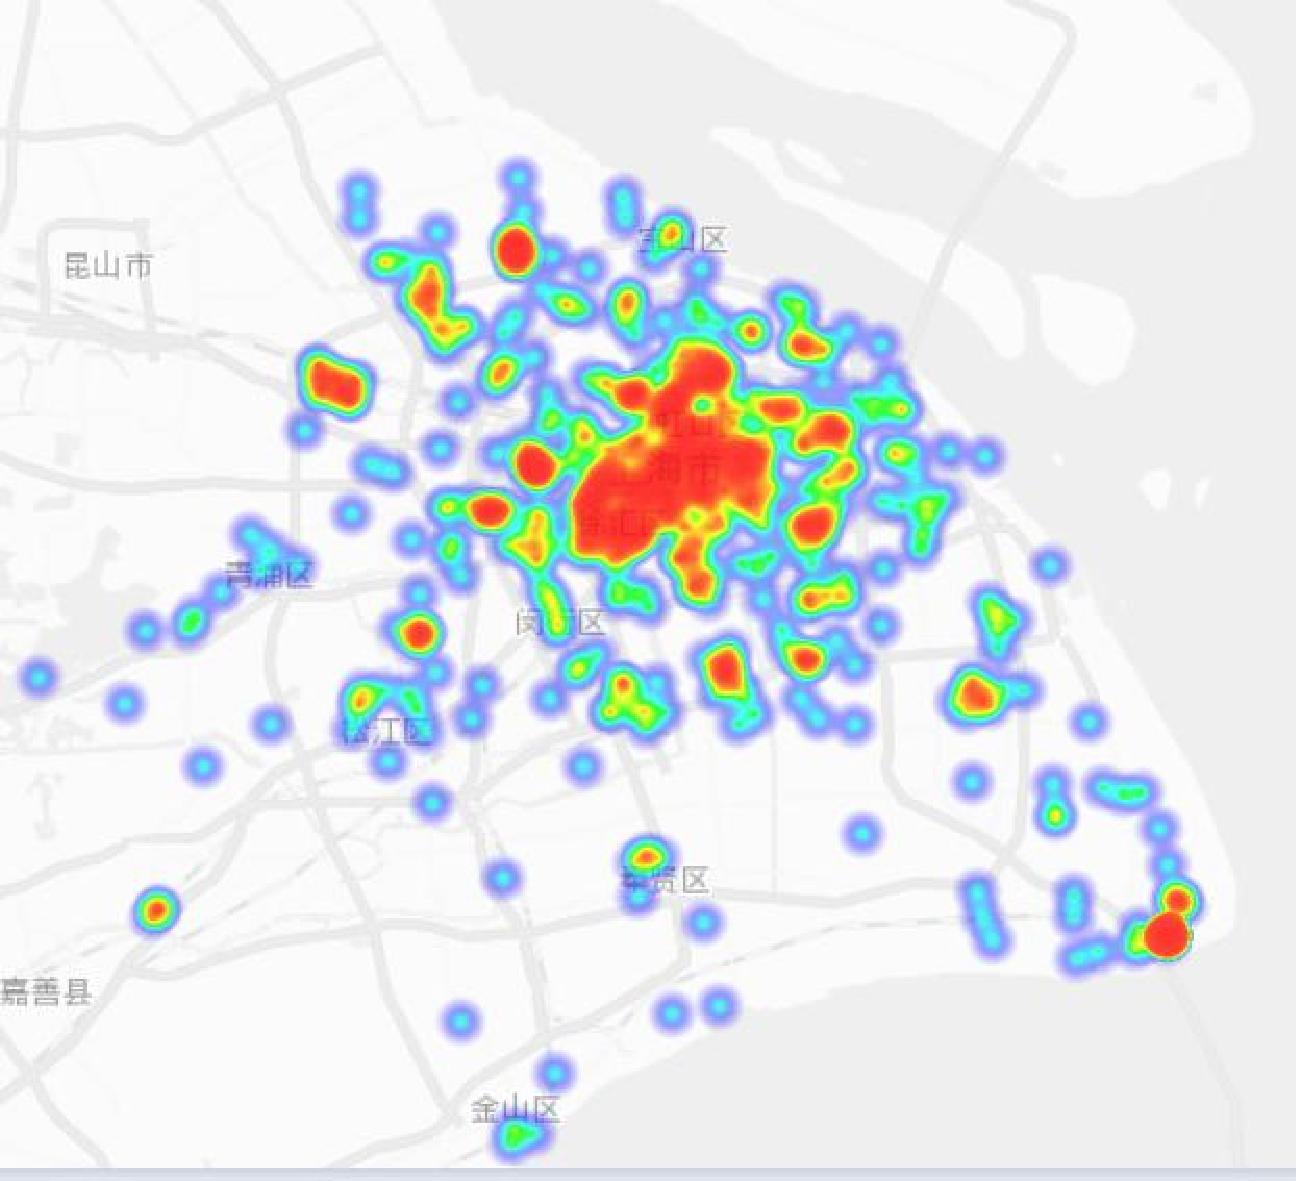
\includegraphics[width=35mm]{weekday.pdf} &  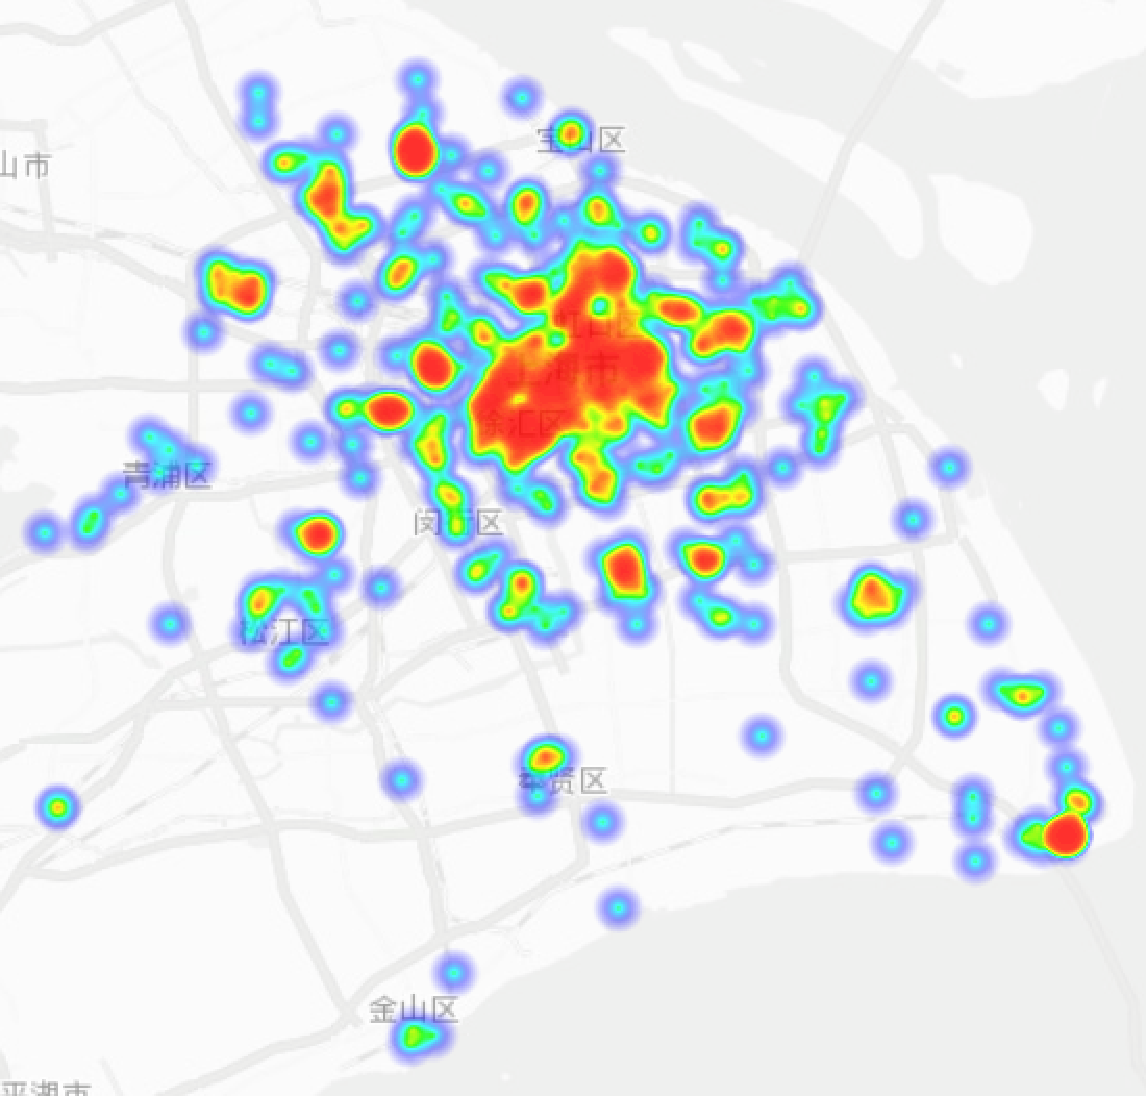
\includegraphics[width=35mm]{weekend.pdf} \\
		(a) Weekdays & (b) Weekends \\[6pt] 
		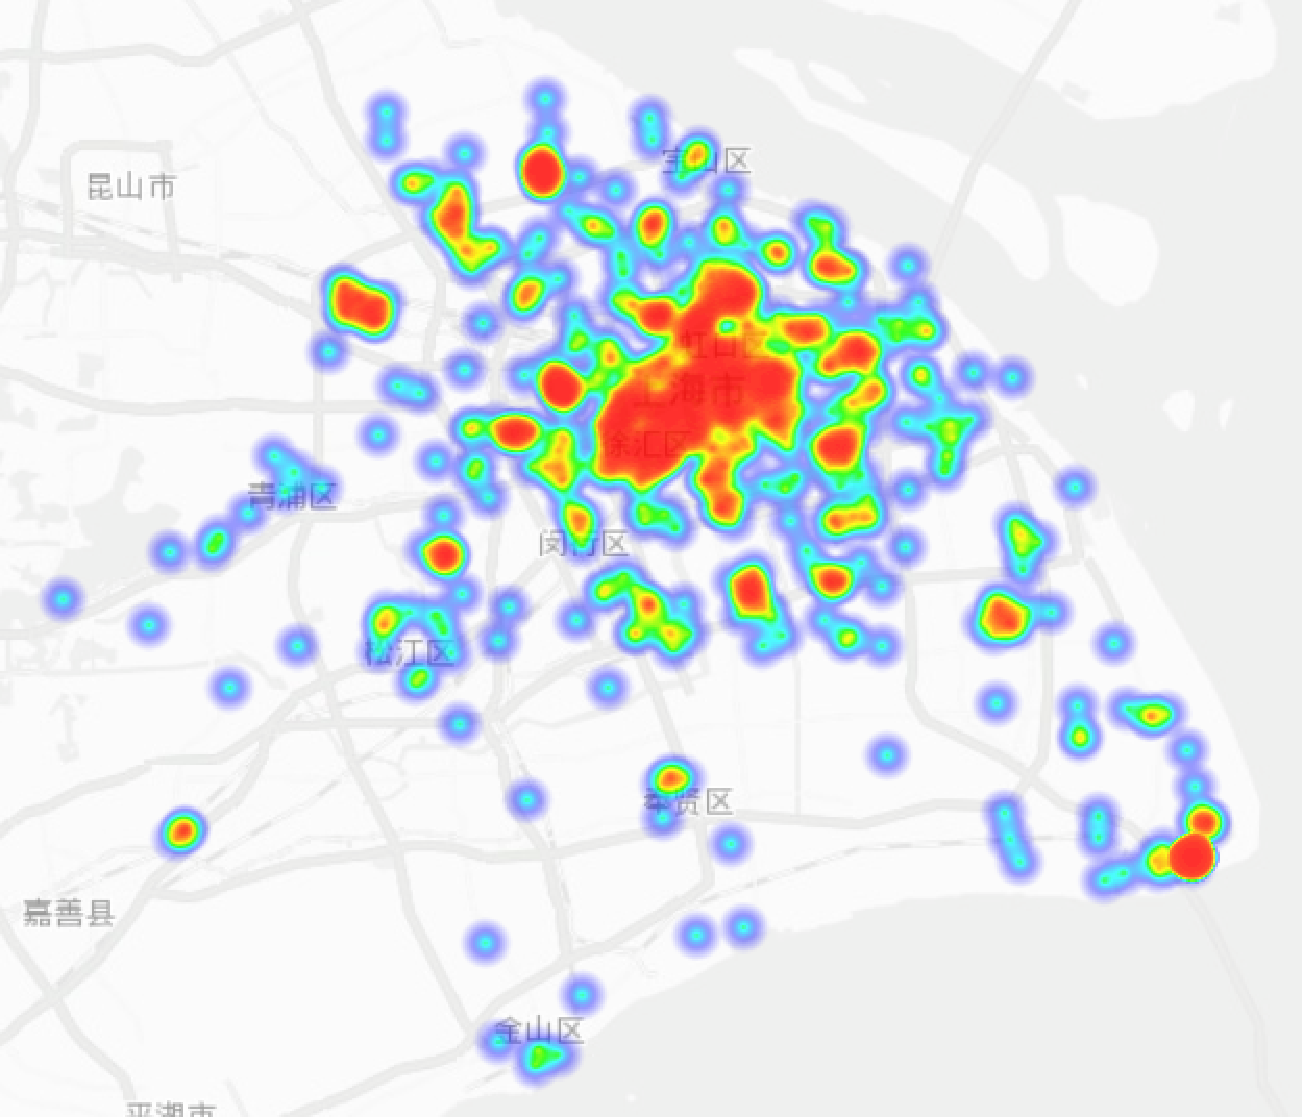
\includegraphics[width=35mm]{morning.pdf} &
		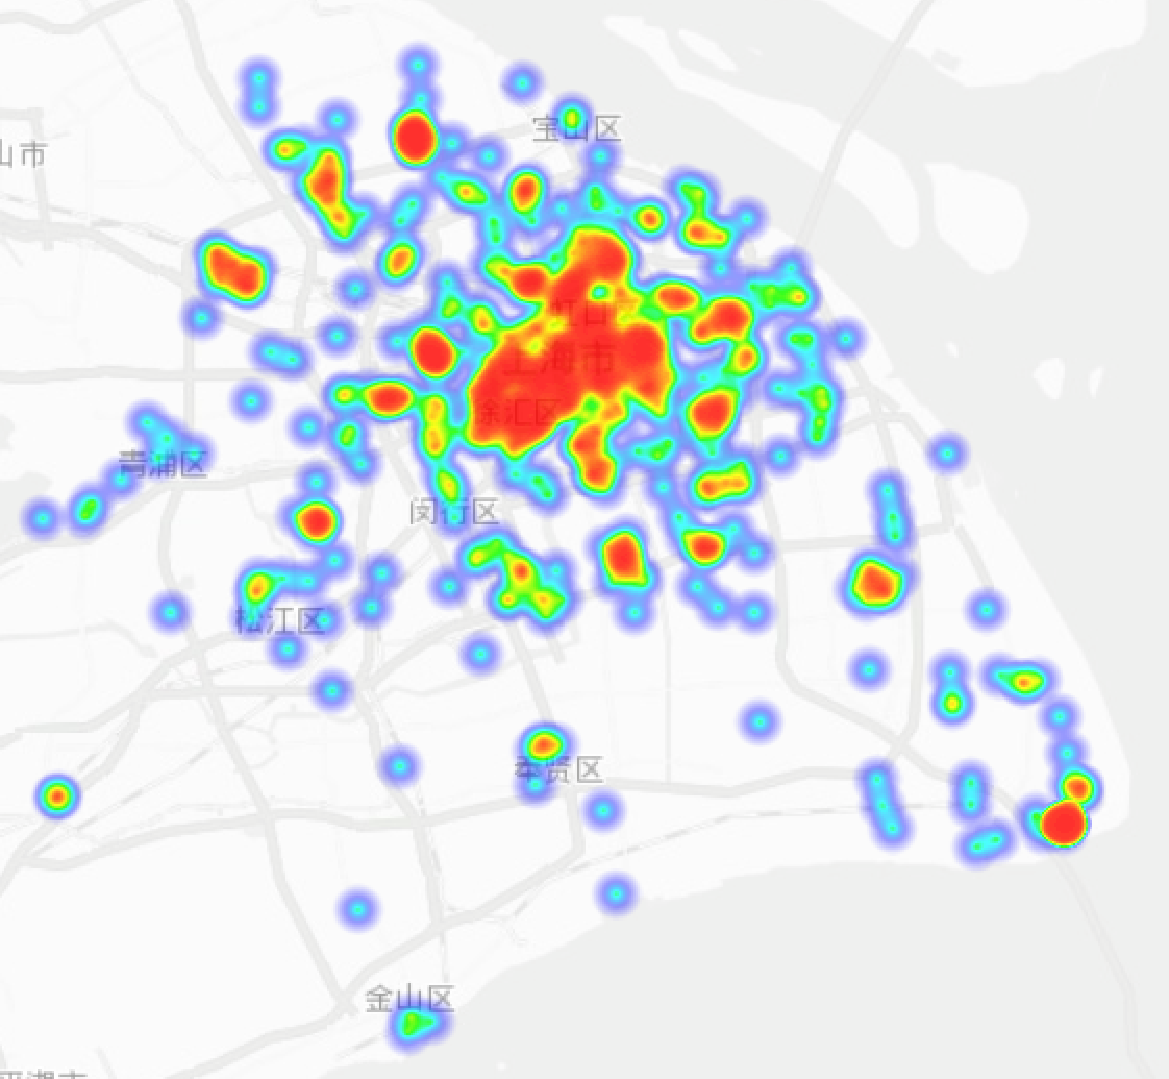
\includegraphics[width=35mm]{evening.pdf} \\
		(c) Mornings & (d) Evenings
	\end{tabular}
	\centering
	\caption{Charging Hotspots in Shanghai in different time frames}
	\label{fig1}
\end{figure}
From Fig.\ref{fig1}, it is easy to notice that in different time frames, the charging hotspots stays at almost the same locations, meaning that during different time periods, the use rate of a given charging station is determined by its spatiotemporal context.

\subsection{Point Of Interest}
To the prosperity of Shanghai, there are so many points of interest(e.g., shopping malls, schools. estates, companies, etc.) located in the city.  Understanding the purpose of the trip by each person who participates in charging system will help us to analyze the use rate prediction. So, we need to extract the POI around each existing charging station. There are a lot of POIs in Shanghai. The POIs are very close to each other. We set a radius around each station and then collect the POIs within the radius. Based on our experiment, choosing a radius as 300 meters is proper. In our work, we get 80 different types of POI totally. Some of the POIs are very similar to each other. Therefore, we group 80 POIs in further step. By grouping POIs, we get 10 groups at last. Table.\ref{tab1} gives the groups and POIs in detail.

\begin{table}[htbp]
	\caption{Groups of POIs}
	\begin{center}
		\begin{tabular}{|l|p{6cm}|}
			\hline
			Group & Points of interests\\
			\hline
			Food & chinese \& foreign restaurant, snack bar, cake \& dessert shop, cafe, bar\\
			\hline
			Hotels & star hotel, express hotel, apartment hotel\\
			\hline
			Shopping & shopping centers, department stores, supermarkets, convenience stores, home building materials, home appliances digital, shops, markets\\
			\hline
			Education & institutions of higher learning, middle schools, primary schools, kindergartens, adult education, parent-child education, special education schools, study agencies, research institutions, training institutions, libraries, science and technology museums\\
			\hline
			Cultural venue & press and publication, radio and television, art groups, art galleries, exhibition halls, cultural palaces\\
			\hline
			Medical & general hospitals, specialist hospitals, clinics, pharmacies, medical examination institutions, nursing homes, emergency centers, disease control centers\\
			\hline
			Car service & car sales, car repair, car beauty, auto parts, car rental, car inspection field\\
			\hline
			Transportation & airport, railway station, subway station, subway line, long-distance bus station, bus station, bus line, port, parking lot, refueling station, service area, toll station, bridge, charging station, roadside parking space\\
			\hline
			Estates & Office building, residential area, dormitory\\
			\hline
		\end{tabular}
		\label{tab1}
	\end{center}
\end{table}

\subsection{Distance}

In use rate prediction, we need to consider distance. People will not choose to park their electric cars for charging if the destination they planned to go is far away. In the system, a station with nearer distance to metro stations, financial centers and major functional buildings would easily be used more often. We select the nearest distance to the following to be the distance we considered as features: company, estate, hospital, metro station, shopping center and university.

\subsection{Price}
By futher digging into the data, we find that there is a 0.3 correlation between price for charging and the use rate. Since there are two types of charging ports: DC and AC. We would include the number of ports and the price of both types in a charging station as one of its feature.

\subsection{Private or public}
By observing the data we've collected, it can be seen that most of the charging stations are private charging stations, which means they are typically used by electric public buses and rent cars, or used by specific companies for their employees, accounting for over 70\% of the total charging stations. Also, since the private are used by more regular users(e.g., buses, companies employees), its use rate are 5\% higher compared to public ones. This alongside other observations will be taken into consideration.

\section{Time Frame Based Model}
\subsection{Time Frames}
We separate the dataset into different time frames, including total time, weekday, weekend, daytime, evening time, morning\_rush hours, evening\_rush hours and travel\_hours.Fig.\ref{fig2} shows the average use-rate of the time frames above.
\begin{figure}[htbp]
	\begin{tabular}{c}
		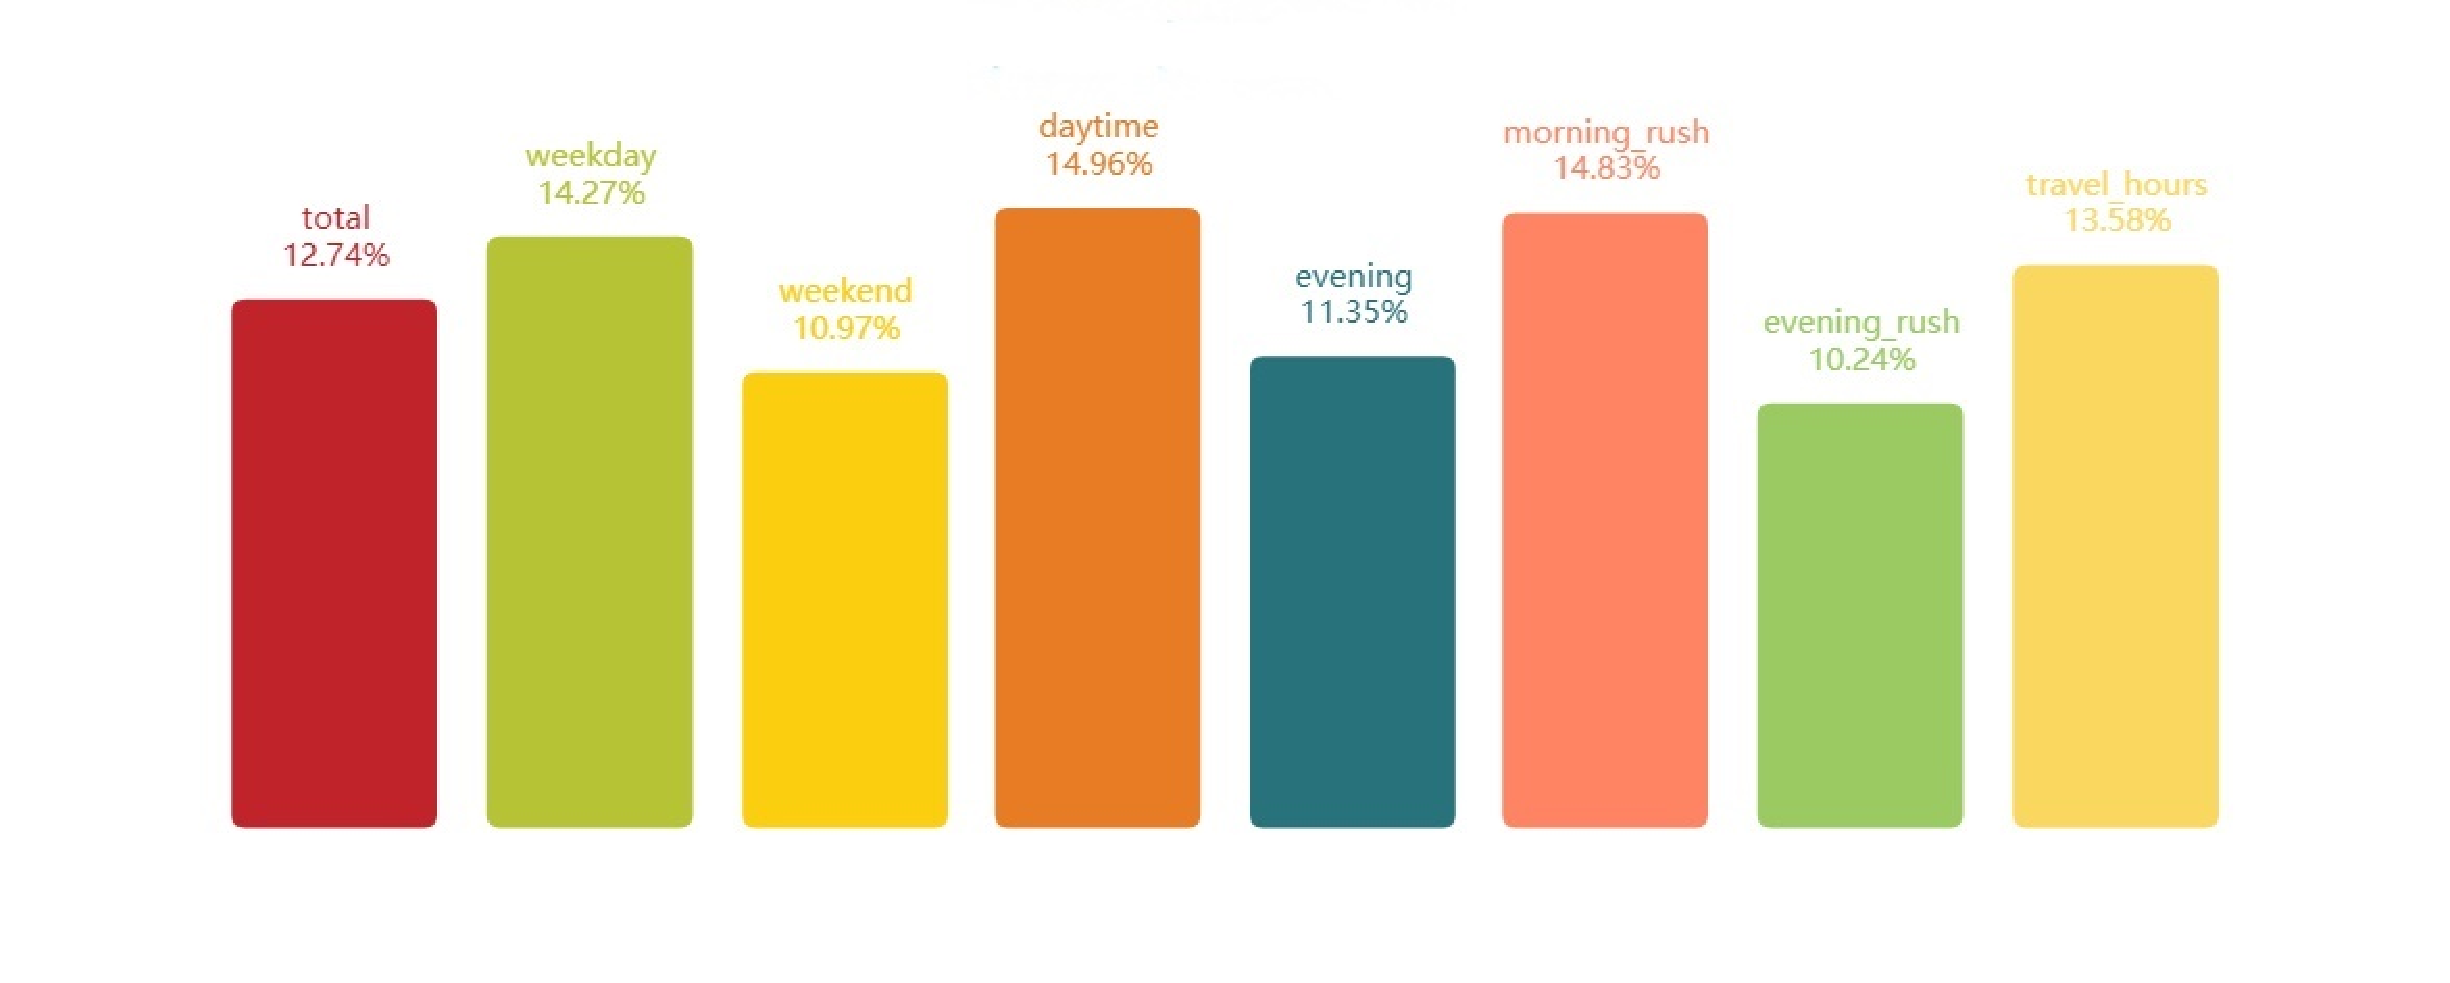
\includegraphics[width=100mm]{timeframes.pdf}
	\end{tabular}
	\centering
	\caption{Average use-rate of different time frames}
	\label{fig2}
\end{figure}

\subsection{Model Description}
In each time frame, we add the geographical information as well as working elements into the prediction model, in order to predict whether it’s a high use\_rate station or a low use\_rate one.
\section{Experiment}

\subsection{Datasets}
In this paper, we gather the charging stations logs from all the existing charging station companies who provide their services in Shanghai, with a total of over 2,000,000 lines. The log has a length of one month, from 2018/10 to 2018/11, in which an hourly summarize of each charging station is recorded, showing whether it's occupied or not. After preprocessing, the training set has 80\% of valid data, the test set has 20\% left.

\subsection{Implementation}

With features extracted from our collected dataset, there are mainly three groups of them, including POIs, charing price and station types, that are added into the time frame based models. Fig.\ref{fig3} shows the general flow path of our work.

\begin{figure}[htbp]
	\begin{tabular}{c}
		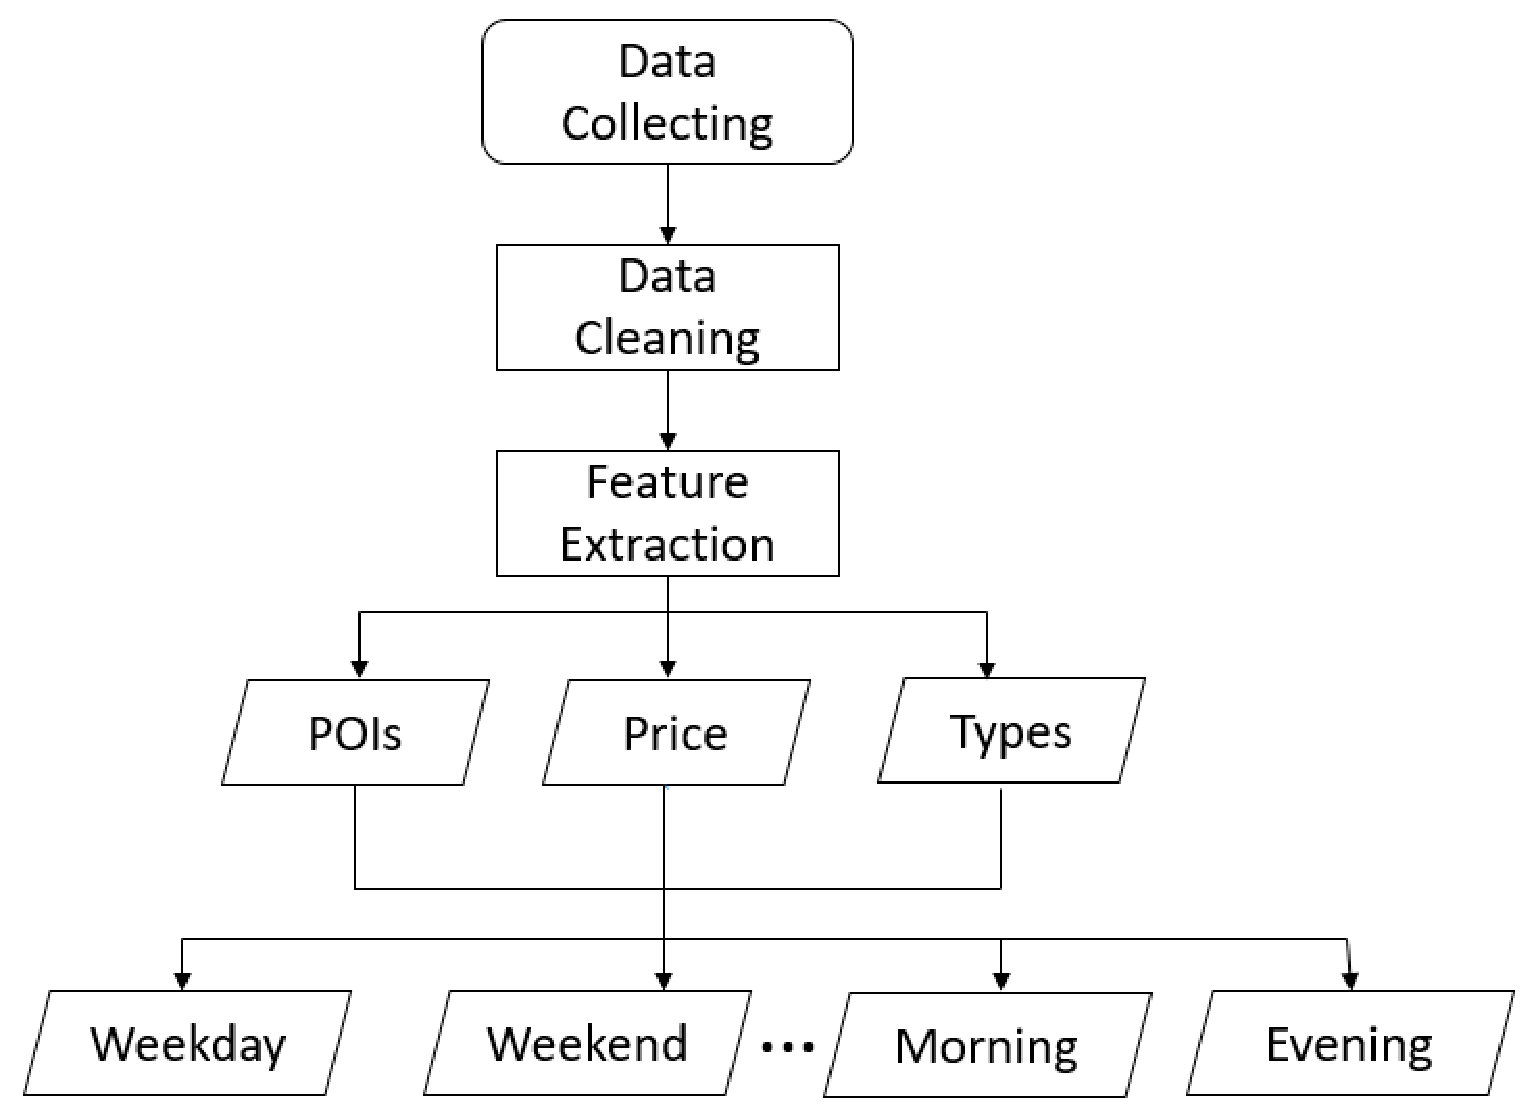
\includegraphics[width=80mm]{path.pdf}
	\end{tabular}
	\centering
	\caption{Implementation of the work}
	\label{fig3}
\end{figure}

\subsection{Results}
We run our dataset on LR, Random Forest, SVM and XGBOOST respectively, along with the features mentioned above added into time frame based models.
\begin{table}[htbp]
	\caption{Evaluation results on different models}
	\begin{center}
		\begin{tabular}{|l|l|}
			\hline
			Model & Accuracy\\
			\hline
			LR & 60.9\%\\
			\hline
			SVMt & 68.9\%\\
			\hline
			Random Forest & 70.1\%\\
			\hline
			XGBOOST & 73.6\%\\
			\hline
		\end{tabular}
		\label{tab2}
	\end{center}
\end{table}
Table.\ref{tab2} shows the prediction accuracy of different models. We can see that they can all perform well based on our settings, and XGBOOST achieves the most favourable result.

\section{Conclusion and Future Work}
In this paper, we propose the time frame based prediction model for use rate of charging stations. We study on some important features like station's surrouding POIs, charing price and station type. In experiments, we separate our dataset into different time frames and add the features into them, which obtains a relatively favourable result, indicating that the use rate of charing station is highly influenced by its geographical information and working elements. Furthermore, it also has a greate impact on location choosing problem.

There is still a lot of work to be continued in the future. First, we only consider three mainly types of features that might affect station use rate, many other important features also need to be extracted and incluede. Furthermore, we might explore a properly modified model to execute those features and gain a more satisfactory result.


\begin{thebibliography}{00}
\bibitem{b1} Jie Bao, Tianfu He, Sijie Ruan, Yanhua Li, and Yu~Zheng.
\newblock Planning bike lanes based on sharing-bikes' trajectories.
\newblock In {\em Proceedings of the 23rd {ACM} {SIGKDD} International
	Conference on Knowledge Discovery and Data Mining, Halifax, NS, Canada,
	August 13 - 17, 2017}, pages 1377--1386, 2017.
\bibitem{b2} Minh~X. Hoang, Yu~Zheng, and Ambuj~K. Singh.
\newblock {FCCF:} forecasting citywide crowd flows based on big data.
\newblock In {\em Proceedings of the 24th {ACM} {SIGSPATIAL} International
	Conference on Advances in Geographic Information Systems, {GIS} 2016,
	Burlingame, California, USA, October 31 - November 3, 2016}, pages 6:1--6:10,
2016.
\bibitem{b3} Yaguang Li, Kun Fu, Zheng Wang, Cyrus Shahabi, Jieping Ye, and Yan Liu.
\newblock Multi-task representation learning for travel time estimation.
\newblock In {\em Proceedings of the 24th {ACM} {SIGKDD} International
	Conference on Knowledge Discovery {\&} Data Mining, {KDD} 2018, London, UK,
	August 19-23, 2018}, pages 1695--1704, 2018.
\bibitem{b4} Yexin Li, Yu~Zheng, and Qiang Yang.
\newblock Dynamic bike reposition: {A} spatio-temporal reinforcement learning
approach.
\newblock In {\em Proceedings of the 24th {ACM} {SIGKDD} International
	Conference on Knowledge Discovery {\&} Data Mining, {KDD} 2018, London, UK,
	August 19-23, 2018}, pages 1724--1733, 2018.
\bibitem{b5} Binbing Liao, Jingqing Zhang, Chao Wu, Douglas McIlwraith, Tong Chen, Shengwen
Yang, Yike Guo, and Fei Wu.
\newblock Deep sequence learning with auxiliary information for traffic
prediction.
\newblock In {\em Proceedings of the 24th {ACM} {SIGKDD} International
	Conference on Knowledge Discovery {\&} Data Mining, {KDD} 2018, London, UK,
	August 19-23, 2018}, pages 537--546, 2018.
\bibitem{b6} Xinyue Liu, Xiangnan Kong, and Yanhua Li.
\newblock Collective traffic prediction with partially observed traffic history
using location-based social media.
\newblock In {\em Proceedings of the 25th {ACM} International Conference on
	Information and Knowledge Management, {CIKM} 2016, Indianapolis, IN, USA,
	October 24-28, 2016}, pages 2179--2184, 2016.
\bibitem{b7} Zhaoyang Liu, Yanyan Shen, and Yanmin Zhu.
\newblock Where will dockless shared bikes be stacked?: - parking hotspots
detection in a new city.
\newblock In {\em Proceedings of the 24th {ACM} {SIGKDD} International
	Conference on Knowledge Discovery {\&} Data Mining, {KDD} 2018, London, UK,
	August 19-23, 2018}, pages 566--575, 2018.
\bibitem{b8} Bilong Shen, Xiaodan Liang, Yufeng Ouyang, Miaofeng Liu, Weimin Zheng, and
Kathleen~M. Carley.
\newblock Stepdeep: {A} novel spatial-temporal mobility event prediction
framework based on deep neural network.
\newblock In {\em Proceedings of the 24th {ACM} {SIGKDD} International
	Conference on Knowledge Discovery {\&} Data Mining, {KDD} 2018, London, UK,
	August 19-23, 2018}, pages 724--733, 2018.
\bibitem{b9} Zidong Yang, Ji~Hu, Yuanchao Shu, Peng Cheng, Jiming Chen, and Thomas
Moscibroda.
\newblock Mobility modeling and prediction in bike-sharing systems.
\newblock In {\em Proceedings of the 14th Annual International Conference on
	Mobile Systems, Applications, and Services, MobiSys 2016, Singapore, June
	26-30, 2016}, pages 165--178, 2016.
\bibitem{b10} Xiao Zhou, Anastasios Noulas, Cecilia Mascolo, and Zhongxiang Zhao.
\newblock Discovering latent patterns of urban cultural interactions in wechat
for modern city planning.
\newblock In {\em Proceedings of the 24th {ACM} {SIGKDD} International
	Conference on Knowledge Discovery {\&} Data Mining, {KDD} 2018, London, UK,
	August 19-23, 2018}, pages 1069--1078, 2018.
\end{thebibliography}
\end{document}
